\begin{center}
    \setcounter{section}{3}
    \setcounter{subsection}{0}
    \section*{CAPÍTULO III}
    \addcontentsline{toc}{section}{MARCO TEÓRICO}
    \vspace*{0.5in}
    \textbf{MARCO TEÓRICO}
\end{center}

\subsection{SCADA}
    ``Es un concepto que se emplea para realizar un software 
    para ordenadores que permite controlar y supervisar 
    procesos industriales a distancia. Facilita 
    retroalimentación en tiempo real con los 
    dispositivos de campo (sensores y actuadores), y 
    controla el proceso automáticamente. Provee de toda 
    la información que se genera en el proceso 
    productivo (supervisión, control calidad, control de
    producción, almacenamiento de datos, etc.) y 
    permite su gestión e intervención." \textcolor{blue}{\cite{SCADA}}\\

    Este tipo de herramienta estan pensadas para la reducción de costos además de la toma de decisiones automaticas o por 
    desición de los supervisores del proceso. Tradicionalmente son elaborados por expertos en lenguaje de bajo nivel 
    al manejar información principalmente proveniente de sensores, el diagrama basico de un sistema SCADA se representa
    en la Figura \ref{fig:estructura} en donde se plantea un esquema en el cual se adquiere información a través de sensores
    y paneles para el operario cumunicandose con un PLC llevando la información a dispositivos HMI o a interfaz usuario. \\

    \begin{figure}[H]
        \centering
        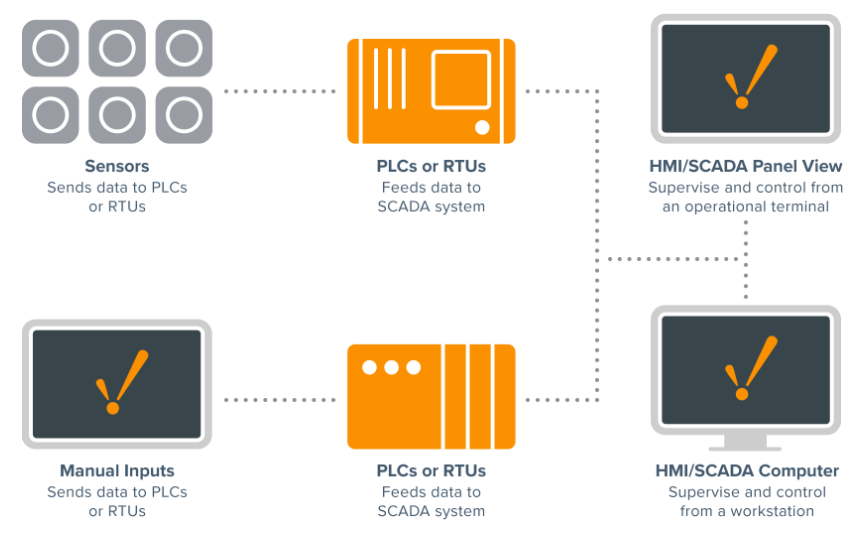
\includegraphics[scale=0.4]
        {EstructuraSCADA.png}
        \caption{Diagrama basico de un sistema SCADA}
    \label{fig:estructura}
    \end{figure}

    Mango Automation ofrece productos de hardware y software para el desarrollo de sistemas SCADA, sin embargo permite que 
    el software se adapte a sistemas ya establecidos realizando la conexión con el software propio del sistema. 

\subsection{Servidor:}
    ``Es un programa informático que procesa una aplicación del lado del servidor, realizando conexiones bidireccionales o unidireccionales y síncronas o asíncronas con el cliente y generando o cediendo una respuesta en cualquier lenguaje o Aplicación del lado del cliente."\textcolor{blue}{\cite{Servidor}}
    
\subsection{Framework:} 
    Es el esquema o estructura que se establece y que se aprovecha para desarrollar y organizar un software determinado.
    ``Un Framework sirve para poder escribir código o desarrollar una aplicación de manera más sencilla. Es algo que permite una mejor organización y control de todo el código elaborado, así como una posible reutilización en el futuro."\textcolor{blue}{\cite{Framework}}
    \\
    Mango Automation implementa AngularJs para el desarrollo de su interfaz como herramienta de desarrollo web permitiendo
    adaptar la interfaz a los requerimientos funcionales y esteticos.
\subsection{Protocolos:} ``En informática y telecomunicación, un protocolo de comunicaciones es un sistema de reglas que permiten que dos o más entidades de un sistema de comunicación se comuniquen entre ellas para transmitir información por medio de cualquier tipo de variación de una magnitud física. Se trata de las reglas o el estándar que define la sintaxis, semántica y sincronización de la comunicación, así como también los posibles métodos de recuperación de errores. Los protocolos pueden ser implementados por hardware, por software, o por una combinación de ambos."\textcolor{blue}{\cite{Protocolo}}
	
\subsection{Escalabilidad:} ``Es un término usado en tecnología para referirse a la propiedad de aumentar la capacidad de trabajo o de tamaño de un sistema sin comprometer el funcionamiento y calidad normales del mismo."\textcolor{blue}{\cite{escalabilidad}}
	
\subsection{Base de datos:} ``Es un conjunto de datos pertenecientes a un mismo contexto y almacenados sistemáticamente para su posterior uso."\textcolor{blue}{\cite{BASE}}
	
%\subsection{LAN:} ``Es una red que conecta los ordenadores en un área relativamente pequeña y predeterminada (como una habitación, un edificio, o un conjunto de edificios)."\textcolor{blue}{\cite{LAN}}
%	
%\subsection{WAN:} ``Red de computadoras que se extiende en una gran franja de territorio, ya sea a través de una ciudad, un país o, incluso, a nivel mundial. "\textcolor{blue}{\cite{WAN}}
	
\subsection{Internet de las cosas (IoT):} ``Agrupación e interconexión de dispositivos y objetos a través de una red (bien sea privada o Internet, la red de redes), dónde todos ellos podrían ser visibles e interaccionar. Respecto al tipo de objetos o dispositivos podrían ser cualquiera, desde sensores y dispositivos mecánicos hasta objetos cotidianos como pueden ser el frigorífico, el calzado o la ropa."\textcolor{blue}{\cite{IOT}}
	
\subsection{Cloud:} ``La computación en la nube son servidores desde Internet encargados de atender las peticiones en cualquier momento. Se puede tener acceso a su información o servicio, mediante una conexión a internet desde cualquier dispositivo móvil o fijo ubicado en cualquier lugar. Sirven a sus usuarios desde varios proveedores de alojamiento repartidos frecuentemente por todo el mundo."\textcolor{blue}{\cite{nube}}
	
\subsection{Interface:} ``Es una conexión entre dos máquinas de cualquier tipo, a las cuales les brinda un soporte para la comunicación a diferentes estratos. Es posible entender la interfaz como un espacio (el lugar donde se desarrolla la interacción y el intercambio)"\textcolor{blue}{\cite{interface}}
    \\

    Se encarga de obtener la información almacenarla y mostrarla de manera mas amigable con el usuario final, idealmente 
    esta debe ser agradable, sencilla además de mostrar data que los usuarios que hacen uso de ella consideren importante.
\subsection{API:} ``Son un conjunto de comandos, funciones y protocolos informáticos que permiten a los desarrolladores crear programas específicos para ciertos sistemas operativos. Las API simplifican en gran medida el trabajo de un creador de programas, ya que no tiene que «escribir» códigos desde cero. Estas permiten al informático usar funciones predefinidas para interactuar con el sistema operativo o con otro programa."\textcolor{blue}{\cite{API}} 
	
\subsection{Mango:} ``Es una aplicación de software multiplataforma basada en web que permite a los usuarios acceder y controlar sensores electrónicos, PLC, controladores, bases de datos o servicios web, a través de múltiples protocolos simultáneamente. Mango proporciona una interfaz con la que se pueden crear y configurar diversas fuentes de datos (data sources), a la vez que proporciona una gestión de accesos a usuarios, registro de datos, alarmas y automatización.\\
	
	Características:
	
	\begin{itemize}
	    \item \textbf{Protocolos integrados:} con BACnet, Modbus, MQTT, SNMP, DNP3, SQL, archivos CSV, HTTP y otros, no es necesario pagar controladores adicionales o herramientas de software. Mango se conectará a todos sus dispositivos y fuentes de datos, integrando todo en una interfaz fácil de usar.
	    
	    \item \textbf{Almacenamiento de datos:} mango es capaz de almacenar billones de valores históricos con un alto rendimiento, mientras utiliza cantidades sorprendentemente pequeñas de espacio en el disco.
	    
	    \item \textbf{Analítica integrada:} mango proporciona varias interfaces web para que los usuarios realicen análisis rápidos y eficientes. Con listas de seguimiento (watch lists) fáciles de configurar y consultas flexibles de datos.
	    
	    \item \textbf{Informes y facturación:} mango proporciona varias interfaces web para que los usuarios realicen análisis rápidos y eficientes. Con listas de seguimiento (watch lists) fáciles de configurar y consultas flexibles de datos.
	    
	    \item \textbf{Horarios y calendarios:} mango cuenta con un planificador que permite programar semanalmente los eventos. También dispone de reglas de excepción que permiten modificar el cronograma predeterminado.
	    
	    \item \textbf{Visualización de datos:}  mango proporciona una plataforma de desarrollo flexible para tableros de control y aplicaciones web/móviles. Con un editor de Drag {\&} Drop, más una vista del código fuente, los usuarios pueden realizar proyectos de manera rápida y eficiente con cualquier nivel de experiencia.
	    
	    \item \textbf{Automatización y alarmas:} mango incluye varios entornos de scripting potentes, que permiten a los usuarios desarrollar cálculos simples o algoritmos de control. Los usuarios pueden configurar varios tipos de alarmas para activar el manejo de eventos o notificaciones, lo que les brinda tranquilidad mientras están ausentes.
	    
	    \item \textbf{APIs}: mango tiene una poderosa arquitectura interna modular (más de 25 módulos de código abierto) que permite a las empresas y desarrolladores crear componentes personalizados. Los módulos pueden ser, desde protocolos hasta aplicaciones completas con sus propios componentes de base de datos."\textcolor{blue}{\cite{MANGO2}}
	    
	\end{itemize}
	
\subsection{MangoES:} ``Es un servidor Linux embebido muy potente basado en ARM con la aplicación completa Mango Enterprise preinstalada. No hay licencias o software adicionales necesarios para operar. Para aplicaciones con menos de 3000 puntos de datos, MangoES reemplaza los costosos servidores con un dispositivo listo para usar. "\textcolor{blue}{\cite{MANGO}}
    

\newpage
